\documentclass[11pt,a4paper]{article}
\usepackage[T1]{fontenc}
\usepackage[utf8]{inputenc}
\usepackage{lmodern}
\usepackage[margin=2.4cm]{geometry}
\usepackage{amsmath,amssymb}
\usepackage{booktabs,tabularx,array}
\usepackage{enumitem}
\usepackage{xcolor}
\usepackage{tikz}
\usetikzlibrary{positioning,arrows.meta}
\usepackage[colorlinks=true,linkcolor=blue!50!black,urlcolor=blue!50!black]{hyperref}

\definecolor{best}{RGB}{20,140,70}
\definecolor{bad}{RGB}{200,40,40}
\newcolumntype{L}{>{\raggedright\arraybackslash}X}
\tikzset{router/.style={circle,draw=blue!60!black,fill=blue!10,thick,minimum size=8mm,font=\bfseries},
         link/.style={thick,gray!70!black},
         w/.style={fill=white,inner sep=1.5pt,font=\small}}

\title{\textbf{IntelliRoute}\\[4pt]\large Dynamic Network Routing and Multi-Criteria Path Optimization}
\author{Member 1 \and Member 2 \and Member 3}
\date{Project plan and technical background}

\begin{document}
\maketitle

\begin{abstract}
IntelliRoute is a Python network simulator that compares three routing strategies on the same
networks and under the same changing conditions: Dijkstra's algorithm with static weights,
Dijkstra's algorithm with dynamically updated weights, and a proposed multi-criteria adaptive
routing method. The project relies only on classical algorithms, graph theory and mathematical
optimization, so that every line can be explained. This document gives the background, states the
research question, describes what will be built and how it will be evaluated, and fixes the
delegation of work between the three team members and the AI assistant.
\end{abstract}

\tableofcontents

\section*{Project summary}
\addcontentsline{toc}{section}{Project summary}
\begin{center}
\fbox{\begin{minipage}{0.94\textwidth}
\textbf{Problem.} Traditional shortest-path calculations based on fixed or limited routing metrics
may not adequately reflect changing network conditions.\\[4pt]
\textbf{Proposed solution.} A software-based routing system that dynamically evaluates network
connections using multiple performance parameters and selects an efficient route through graph
algorithms.\\[4pt]
\textbf{Core technologies.} Graph theory; Dijkstra's algorithm; multi-criteria optimization;
dynamic edge-weight calculation; Python network simulation.\\[4pt]
\textbf{Expected outcome.} A working application that demonstrates how adaptive multi-criteria
routing behaves under changing network conditions and whether it improves performance over
conventional approaches.
\end{minipage}}
\end{center}

\section{What is routing?}
A computer network is a set of \emph{routers} joined by \emph{links}. Data does not travel in one
piece: it is cut into small units called \emph{packets}. When a computer sends a packet to a
server, the packet crosses several routers; each router looks at the destination and decides where
to forward the packet next. \emph{Routing} is the problem of deciding which sequence of links the
packets should follow.

A useful picture: routers are cities, links are roads and packets are cars. Routing is choosing the
roads.

\begin{center}
\begin{tabular}{ll}
\toprule
Term & Meaning \\
\midrule
Router & a device that receives packets and forwards them \\
Link & a connection between two routers \\
Packet & a small unit of data \\
Path (route) & a sequence of links from a source to a destination \\
\bottomrule
\end{tabular}
\end{center}

\section{The problem}
Suppose data must go from router $A$ to router $F$ and three paths exist:
$A\to B\to D\to F$, $A\to C\to E\to F$ and $A\to B\to E\to F$.
The path with the fewest links is not necessarily the best one. One path may be short but contain a
congested link; another may be longer but fast on every link; a third may be the shortest but lose
packets. \emph{Shortest}, \emph{fastest} and \emph{most reliable} are three different things.

\paragraph{Research question.}
\begin{quote}
\itshape How can we dynamically select the most efficient route for data packets by considering
multiple network performance parameters instead of relying solely on the shortest path?
\end{quote}

\section{Dijkstra's algorithm}
\subsection{Model}
The network is a weighted graph $G=(V,E)$: $V$ is the set of routers, $E$ the set of links, and each
link $(u,v)$ has a cost $c(u,v)\ge 0$. The cost of a path is the sum of the costs of its links.
Dijkstra's algorithm (Edsger W.~Dijkstra, 1956) finds, from a source $s$, a path of lowest total
cost to every other node.

\subsection{Worked example}
\begin{figure}[h]
\centering
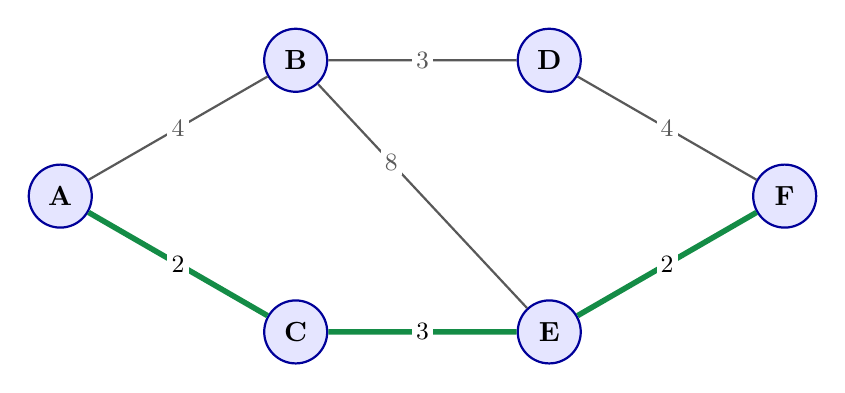
\begin{tikzpicture}[scale=1.15]
\node[router] (A) at (0,0) {A};
\node[router] (B) at (2.6,1.5) {B};
\node[router] (C) at (2.6,-1.5) {C};
\node[router] (D) at (5.4,1.5) {D};
\node[router] (E) at (5.4,-1.5) {E};
\node[router] (F) at (8,0) {F};
\draw[link] (A)--node[w]{4}(B);
\draw[link] (B)--node[w]{3}(D);
\draw[link] (D)--node[w]{4}(F);
\draw[link] (B)--node[w,pos=0.35]{8}(E);
\draw[best,line width=2pt] (A)--node[w,text=black]{2}(C);
\draw[best,line width=2pt] (C)--node[w,text=black]{3}(E);
\draw[best,line width=2pt] (E)--node[w,text=black]{2}(F);
\end{tikzpicture}
\caption{Example network. The lowest-cost path from $A$ to $F$ is shown in green.}
\label{fig:graph}
\end{figure}

\begin{center}
\begin{tabular}{lcl}
\toprule
Path & Computation & Total cost \\
\midrule
$A\to B\to D\to F$ & $4+3+4$ & $11$ \\
$A\to C\to E\to F$ & $2+3+2$ & \textbf{7} \\
$A\to B\to E\to F$ & $4+8+2$ & $14$ \\
\bottomrule
\end{tabular}
\end{center}

The best path is $A\to C\to E\to F$ with cost $7$.

\subsection{How it works}
Every node $v$ keeps a tentative distance $d(v)$, initially $d(s)=0$ and $d(v)=\infty$ otherwise.
The algorithm repeatedly picks the unvisited node $u$ with the smallest distance and \emph{relaxes}
its outgoing links:
\[
  d(v)\;\leftarrow\;\min\bigl(d(v),\; d(u)+c(u,v)\bigr).
\]

\begin{center}
\fbox{\begin{minipage}{0.92\textwidth}
\textbf{Algorithm 1: Dijkstra's algorithm}\\[2pt]
\textbf{Input:} graph $G=(V,E)$, costs $c\ge 0$, source $s$.\quad
\textbf{Output:} distances $d$ and predecessors $\pi$.
\begin{enumerate}[label=\arabic*:,itemsep=1pt,topsep=4pt,leftmargin=2em]
\item $d(s)\leftarrow 0$;\quad $d(v)\leftarrow\infty$ for all $v\neq s$;\quad $Q\leftarrow V$
\item \textbf{while} $Q\neq\emptyset$ \textbf{do}
\item \quad $u\leftarrow$ node of $Q$ with smallest $d(u)$;\quad remove $u$ from $Q$
\item \quad \textbf{for each} neighbour $v$ of $u$ still in $Q$ \textbf{do}
\item \quad\quad \textbf{if} $d(u)+c(u,v)<d(v)$ \textbf{then}
\item \quad\quad\quad $d(v)\leftarrow d(u)+c(u,v)$;\quad $\pi(v)\leftarrow u$
\item \textbf{return} $d,\pi$
\end{enumerate}
\end{minipage}}
\end{center}

On the example, the visiting order and the distances are:

\begin{center}
\begin{tabular}{clcccccc}
\toprule
Step & Node picked & $d(A)$ & $d(B)$ & $d(C)$ & $d(D)$ & $d(E)$ & $d(F)$ \\
\midrule
0 & --  & 0 & $\infty$ & $\infty$ & $\infty$ & $\infty$ & $\infty$ \\
1 & $A$ & 0 & 4 & 2 & $\infty$ & $\infty$ & $\infty$ \\
2 & $C$ & 0 & 4 & 2 & $\infty$ & 5 & $\infty$ \\
3 & $B$ & 0 & 4 & 2 & 7 & 5 & $\infty$ \\
4 & $E$ & 0 & 4 & 2 & 7 & 5 & 7 \\
5 & $D$ & 0 & 4 & 2 & 7 & 5 & 7 \\
\bottomrule
\end{tabular}
\end{center}

\paragraph{Correctness and complexity.}
When all costs are non-negative, the distance of a node is final at the moment it is picked, so the
result is optimal. With a binary heap the running time is $O\bigl((|V|+|E|)\log|V|\bigr)$.

\subsection{Limitation}
Dijkstra's algorithm computes the best path \emph{for the weights it is given}. Suppose congestion
raises the cost of link $A$--$C$ from $2$ to $15$. The old route $A\to C\to E\to F$ now costs
$15+3+2=20$, and the best route becomes $A\to B\to D\to F$ with cost $11$. The algorithm only finds
this if someone updates the weights and runs it again. It does not monitor the network, and it does
not say how latency, loss, bandwidth and congestion should be turned into a single cost. These two
gaps are the subject of the project.

\section{Proposed approach: multi-criteria adaptive routing}
\emph{The exact model is a design choice of the team; the formulation below is the starting
proposal and will be refined during the project.}

\subsection{Link cost}
Each link $(i,j)$ is described at time $t$ by its latency $L_{ij}(t)$, packet-loss rate
$P_{ij}(t)$, available bandwidth $B_{ij}(t)$ and congestion (utilisation) $U_{ij}(t)$. Each quantity
is normalised to $[0,1]$ (written with a hat) and combined into one non-negative cost:
\begin{equation}
  c_{ij}(t) \;=\; w_1\,\hat L_{ij}(t) \;+\; w_2\,\hat P_{ij}(t)
  \;+\; w_3\,\bigl(1-\hat B_{ij}(t)\bigr) \;+\; w_4\,\hat U_{ij}(t),
  \qquad w_k\ge 0,\quad \sum_{k=1}^{4} w_k = 1 .
  \label{eq:cost}
\end{equation}
The weights $w_k$ express what is being optimised (for example, a larger $w_2$ for traffic that
cannot tolerate loss). Because $c_{ij}(t)\ge 0$, Dijkstra's algorithm remains valid on these costs.

\subsection{Adaptation}
Costs are recomputed whenever conditions change (or at a fixed interval), and the best path is
recomputed. To avoid switching back and forth between two nearly equal routes (\emph{route
flapping}), the current route $R$ is replaced by a new route $R'$ only if the improvement is
significant:
\begin{equation}
  \mathrm{cost}(R') \;<\; (1-\delta)\,\mathrm{cost}(R), \qquad 0<\delta<1 .
  \label{eq:hyst}
\end{equation}
A failed router or link is modelled by removing it from the graph (infinite cost).

\section{What will be built}
A network simulator written in Python, in four parts.

\begin{description}[leftmargin=1.2cm,style=nextline]
\item[A. Topology editor] Create routers, connect them, assign properties to each connection, and
select the source and the destination.
\item[B. Condition simulator] Change the network over time: congestion, latency, bandwidth, packet
loss and router failures.
\item[C. Routing engine] Three strategies run on the same network:
  (1) Dijkstra with static weights;
  (2) Dijkstra with dynamically updated weights;
  (3) the proposed multi-criteria adaptive routing.
\item[D. Results dashboard] Selected route, total cost, average latency, packet delivery ratio,
number of route changes, and a performance comparison of the three strategies.
\end{description}

\section{Evaluation plan}
The claim that the proposed method is better must be supported by experiments.

\begin{itemize}[leftmargin=*]
\item \textbf{Scenarios.} 100 simulated scenarios (topologies and sequences of condition changes),
generated with fixed random seeds so that they can be reproduced.
\item \textbf{Fairness.} The three strategies are run under identical conditions in every scenario.
\item \textbf{Stronger baseline.} The proposed method is also compared with ordinary Dijkstra using
updated latency weights, to check that using several criteria really adds value over a single
well-chosen one.
\item \textbf{Metrics.}
\end{itemize}

\begin{center}
\begin{tabularx}{\textwidth}{lL}
\toprule
Metric & Definition \\
\midrule
Average latency & mean end-to-end delay of delivered packets \\
Packet delivery ratio & packets delivered $/$ packets sent \\
Throughput & data delivered per unit of time \\
Route computation time & time needed to compute a route \\
Route changes & number of times the selected route changes during a scenario \\
\bottomrule
\end{tabularx}
\end{center}

Results are reported as means over the 100 scenarios with a measure of spread, and no conclusion is
written before the corresponding numbers exist.

\section{Delegation plan}
\subsection{Principles}
The split follows two kinds of awareness.

\begin{itemize}[leftmargin=*]
\item \textbf{Problem awareness} -- knowing what has to be tackled and what the final result must
look like: a working simulator, three comparable routing strategies, experimental evidence, and a
team able to explain every line to the professor.
\item \textbf{Platform awareness} -- knowing what the AI assistant can and cannot do. It is fast at
drafting code skeletons, unit tests, \LaTeX{} and diagrams, and at explaining concepts. It can also
be confidently wrong, it cannot run or observe our simulator unless we give it the output, and it
cannot take responsibility for a result.
\end{itemize}

\subsection{Who does what}
\begin{center}
\begin{tabularx}{\textwidth}{>{\bfseries}p{2.5cm}LL}
\toprule
Owner & Responsibilities & Deliverables \\
\midrule
Member 1\newline Algorithms &
Graph model; Dijkstra with static weights; Dijkstra with updated weights; multi-criteria cost
\eqref{eq:cost} and switching rule \eqref{eq:hyst}; correctness tests on small hand-checked graphs &
Routing engine (part C); explanation of the algorithms for the oral \\
\addlinespace
Member 2\newline Simulator &
Topology editor; condition simulator (congestion, latency, bandwidth, loss, failures); packet
simulation loop; dashboard &
Parts A, B and D; user guide \\
\addlinespace
Member 3\newline Experiments and report &
Scenario generator with seeds; metric collection; running the 100 scenarios; plots and statistics;
\LaTeX{} report and slides &
Result tables and figures; final report \\
\addlinespace
AI assistant &
First drafts of code skeletons, unit tests, \LaTeX{} tables and figures; explanations of concepts;
review of code and text on request &
Drafts only -- nothing is final until its human owner has checked it \\
\bottomrule
\end{tabularx}
\end{center}

\subsection{What is delegated to the AI and what is not}
\begin{center}
\begin{tabularx}{\textwidth}{LLL}
\toprule
Task & AI role & Human check \\
\midrule
Code skeletons, helper functions, unit tests & drafts & owner reads every line, runs the tests, and
can explain the code without the AI \\
Explaining Dijkstra, relaxation, complexity & tutor & checked against the worked example and a
textbook \\
\LaTeX{} layout, tables, TikZ figures & drafts & Member 3 compiles and verifies every number \\
Choosing the cost model and the weights & suggests options & decided and justified by the team \\
Running experiments, measuring results & none & done by the team on the real simulator \\
Interpreting results, writing conclusions & may rephrase text & every claim must be traceable to a
measured result \\
\bottomrule
\end{tabularx}
\end{center}

\paragraph{Rules.}
(1) Every AI output has a human owner. (2) Nothing enters the repository or the report unless its
owner can explain it. (3) The AI never supplies experimental numbers. (4) AI assistance is
acknowledged in the report.

\subsection{Shared work and integration}
The interface between the parts is fixed first, by the whole team: a common graph data structure and
a function \texttt{route(graph, source, destination)} that every strategy implements. Each member
reviews one other member's work (1 reviews 2, 2 reviews 3, 3 reviews 1), and the whole team rehearses
the oral explanation.

\section{Development roadmap}
The project is built in stages rather than by writing hundreds of lines of code at once. Each stage
ends with something that works and that the whole team understands.

\begin{center}
\begin{tabularx}{\textwidth}{c>{\raggedright\arraybackslash}p{3.3cm}Lp{2.6cm}}
\toprule
Stage & Name & Content & Lead \\
\midrule
1 & Networking fundamentals & Routers, packets, topology, routing tables, links and graph
representation & all \\
2 & Classical algorithms & Implement Dijkstra; understand its complexity and limitations &
Member 1 \\
3 & Network cost model & Design and normalise the latency, congestion, bandwidth and packet-loss
measurements & Member 1, with Member 3 \\
4 & Dynamic routing & Automatic cost updates, route recalculation and hysteresis & Member 1, with
Member 2 \\
5 & Simulation and interface & Build the network topology, introduce changing conditions and
visualise packet routes & Member 2 \\
6 & Experiments & Compare the algorithm with conventional approaches, analyse the results and
identify improvements & Member 3 \\
\bottomrule
\end{tabularx}
\end{center}
The report is written in \LaTeX{} throughout the project (Member 3), not at the end.

\section{Limitations}
\begin{itemize}[leftmargin=*]
\item \textbf{The weighted cost is a compromise.} Minimising \eqref{eq:cost} does not guarantee
that the selected route is simultaneously the fastest, the most reliable and the highest-bandwidth
route. The weights encode which trade-offs the team considers acceptable, and this choice must be
stated and justified.
\item \textbf{The simulator demonstrates an algorithmic solution.} It does not change the routing
tables of real ISP routers; that would require additional networking protocols and infrastructure.
\item \textbf{Results hold for the simulated scenarios.} Conclusions are limited to the topologies
and condition models that were tested.
\end{itemize}

\section{Conclusion}
Dijkstra's algorithm gives the optimal path for a given set of weights, but a real network changes
and has more than one quality criterion. IntelliRoute keeps the classical algorithm, feeds it a
multi-criteria cost that follows the state of the network, and measures on 100 identical scenarios
whether this really improves latency, delivery ratio and stability.

\end{document}
